\chapter{Background} \label{chap:background}
% -------------------------
%% QUOTE
\vspace*{\fill}
\epigraph{The more we learn about the world, and the deeper our learning, the more conscious, specific, and articulate will be our knowledge of what we do not know, our knowledge of our ignorance.\\ For this, indeed, is the main source of our ignorance — the fact that\\ \textbf{our knowledge can be only finite, while our ignorance must necessarily be infinite.}}%
{\textit{Conjectures and Refutations (1963)}\\ \textsc{Karl Popper}}
\clearpage{\thispagestyle{empty}\cleardoublepage}
%%
%% Body of the chapter
%%%%%%%%%%%%%%%%%%%%%%
\section{Nanogels from polyelectrolyte complexes}


\section{Transport of polymer and nanoparticles in porous media}
The transport of water additives in porous media is governed by the phenomena retention, adsorption and inaccessible pore volume (IPV) as described by \citep{Lotsch1985}. Changes in composition of the injected solution (e.g., polymer, nanoparticles, salt concentration) affect the responses measured by various sensors. Figure 5.1 shows a few idealized cases of such responses. An ideal piston-like plug flow would look like a step function. However, the real-world effect from dispersion reforms the step function into a curve.

Inaccessible pore volume and retention can shift the curve in Figure \ref{fig:ipvRet1}. The portion of the porous media that cannot be accessed by the particle under study (e.g., the polymer) is referred to as inaccessible pore volume (IPV). The reduced accessible pore volume results in a faster transport of the particles across the porous medium and therefore shifts the response curve to the left. On the other hand, some of the particles under study can be adsorbed on the surface of the rock (adsorption) or are stuck and filtered in small pore throats (mechanical entrapment). These effects delay particle flow through porous media, which are collectively referred to as retention. As a result, the response curve is shifted to the right. 

One should only expect the effect of dispersion on responses for step changes in the salt concentration. However, polymer and nanoparticle responses can experience any combination of effects from dispersion, IPV, retention, and flooding history.

\begin{figure}[h!]
    \centering
    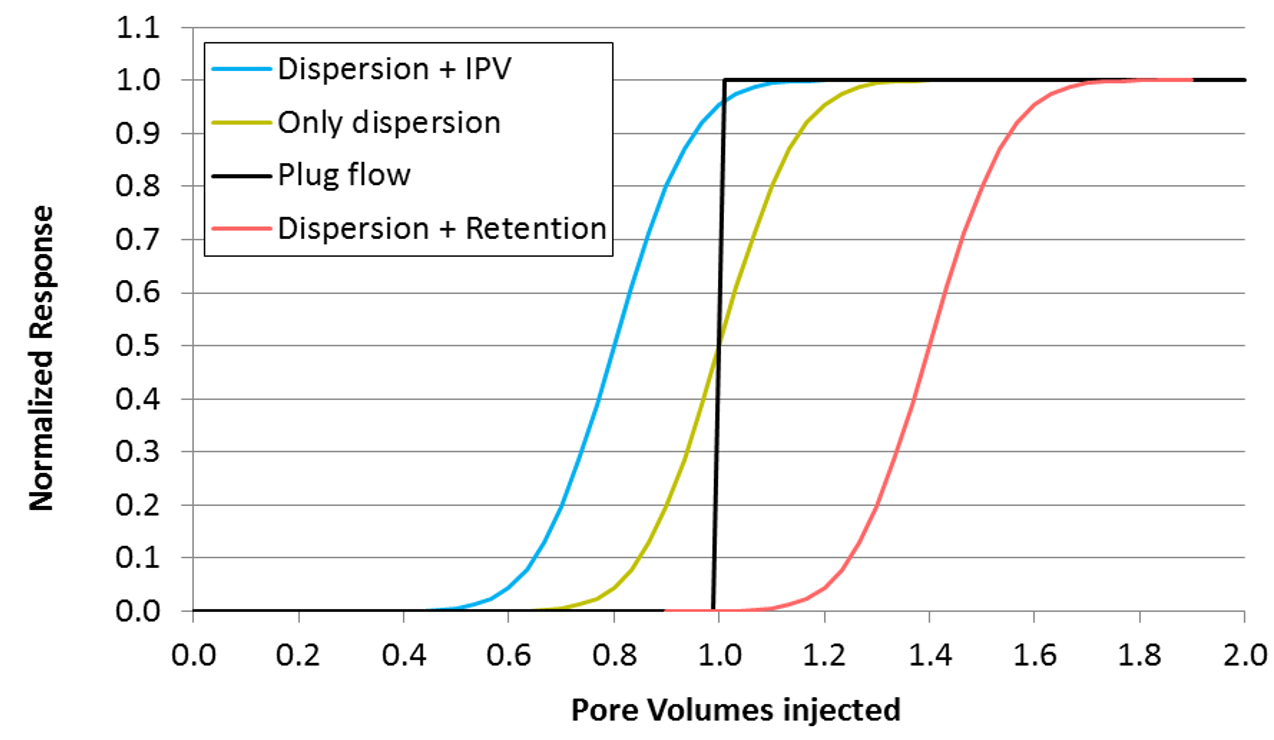
\includegraphics[width=\textwidth]{img/fig/ipvRet1.png}
    \caption{Effect of dispersion, inaccessible pore volume (IPV) and retention on relative responses.}
    \label{fig:ipvRet1} % 5.1
\end{figure}

In order to determine inaccessible pore volume of e.g., polymer, one can compare the production profiles of polymer and a tracer as a function of pore volumes injected. Figure \ref{fig:ipvRet2} illustrates such a comparison. The relative response of polymer is the ratio of measured effluent concentration to the injected concentration. The tracer should ideally have no IPV, i.e., the area below the tracer response should be equal to one. Changing the concentration in salt tracer will yield a close enough response. The area between the two responses determines the IPV.

\begin{figure}[h!]
    \centering
    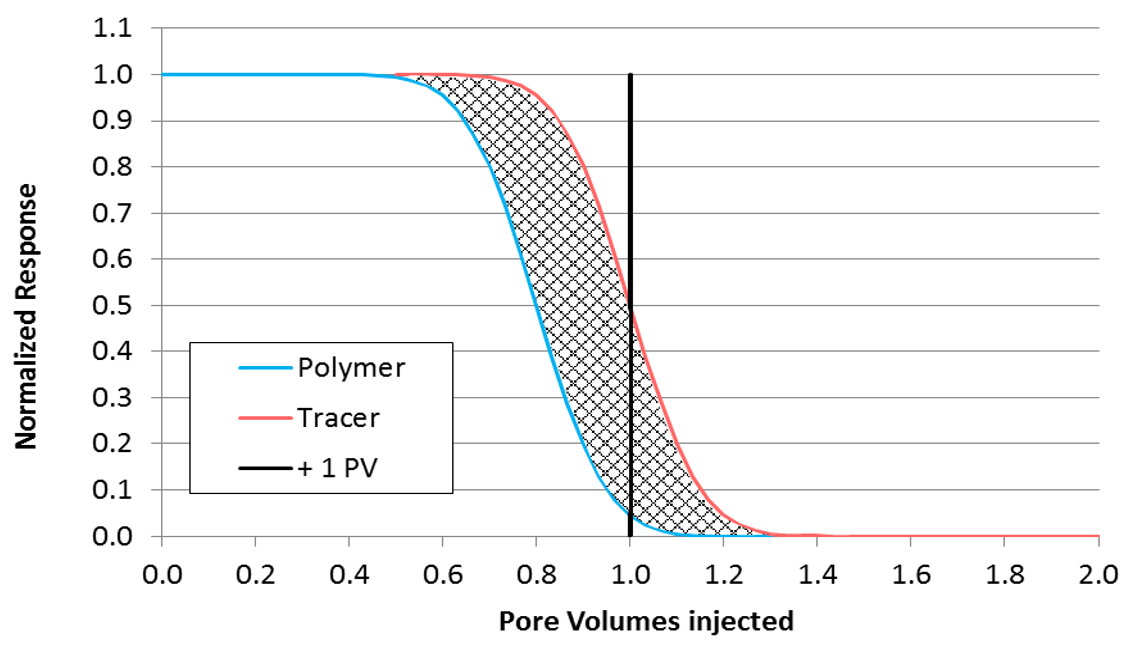
\includegraphics[width=\textwidth]{img/fig/ipvRet2.png}
    \caption{Effect of dispersion, inaccessible pore volume (IPV) and retention on relative responses.}
    \label{fig:ipvRet2} % 5.2
\end{figure}

Provided that the adsorption of polymer is irreversible and no mechanically entrapped polymer is released during water injection, the IPV will result in a response curve with an area under the curve of less than 1. Thus, IPV for polymer will be a positive value. However, if the system experiences desorption of the mechanically entrapped component, the area under the curve may become larger than the tracer area, resulting in a negative IPV indicating release of retained component. 

Total retention of a component in the rock depends on adsorption and mechanical entrapment. A multi-slug experiment can be used to quantify adsorption. Assuming that adsorption for the component under study were irreversible, all the adsorption happened in the first slug, i.e., no more adsorption took place during the second slug, and the magnitude of mechanical entrapment in both slugs were equal, one can compare the relative responses from the two slugs to find adsorption for the component. This is illustrated in Figure \ref{fig:ipvRet3}.

\begin{figure}[h!]
    \centering
    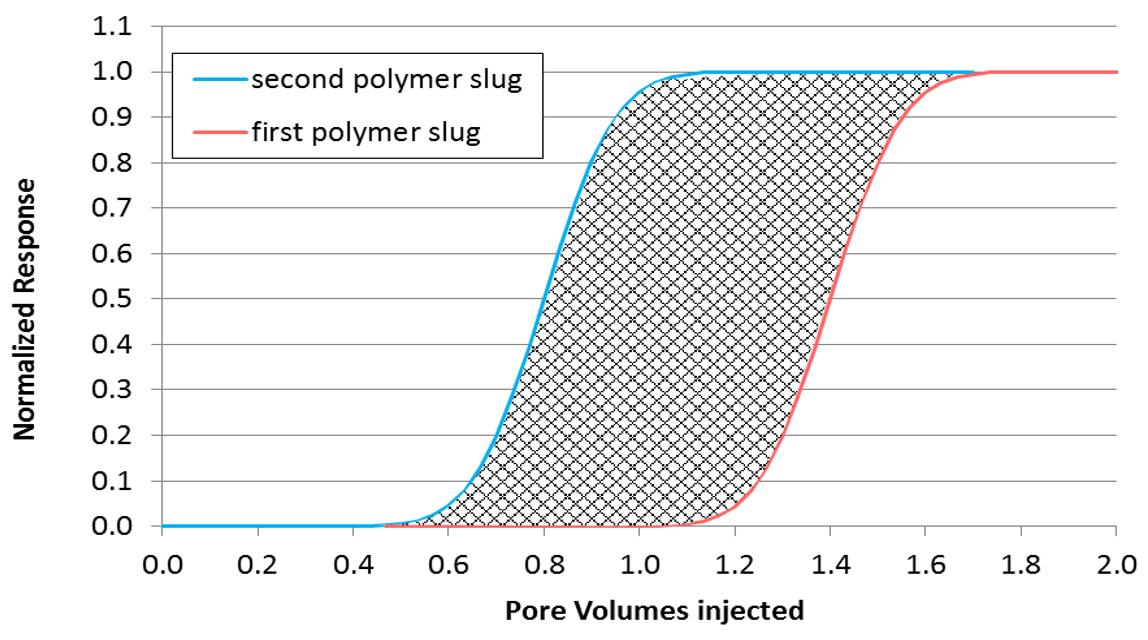
\includegraphics[width=\textwidth]{img/fig/ipvRet3.png}
    \caption{Effect of dispersion, inaccessible pore volume (IPV) and retention on relative responses.}
    \label{fig:ipvRet3} % 5.3
\end{figure}